% Physics of the unified abstract model

\section[Action Potential]{Action Potential\label{sec:Physics-ActionPotential}}

The distinguished role of \gls{AP} deserves a separate section.
A smaller number of non-gated ion channels is distributed over the surface of the membrane, and the overwhelming majority of ion channels is concentrated in the \gls{AIS}.


\subsection{The physical process\label{sec:AP-PhysicalProcess}}

In the resting state, we have a condenser that has some low-conductance resistors (the resting ion channels) across its plate and a very low intensity (nearly constant) distributed current flows, under the effect of a slightly varying (nearly constant) membrane voltage. Due to the membrane potential, a current through the always-open channels flows on the dendritic surface
and the resting channels' conductivity represents a drain with 
sufficient transmission. The resting current practically does not 
reach the \gls{AIS}: the ion channels along the current's path
practically "shunt" the current.
This is a static state that classic neuroscience assumes: some static current in and some static (leakage) current out; no significant gradient.
\textit{In this state}, an almost correct model is a condenser with a
\textit{parallelly} switched resistor; an integrator-type  $RC$ circuit
(although when approaching the threshold voltage, the \gls{AIS} plays some role. The smaller gradient changes, such as subthreshold excitations, produce "mini-\gls{AP} waves"~\cite{NeuralEnergyConsumption:2017}, providing direct experimental proof that in this state the parallel $RC$ circuit is not correct).
The small perturbations are counterbalanced, but their
amount does not exceed a predefined threshold.

In the transient (perturbed) state, the process variable
(the membrane's potential) exceeds the threshold. That event acts
as a fast trigger signal. The amount of charged particles (and so:
the membrane's voltage) suddenly increases, the created gradient
drives a current.
When $Na^+$ ions rush into the intracellular layer, they roughly increase the overall concentration and the potential in that thin layer.
All other ions, including $K^+$, also feel a driving force. The targeted membrane potential is set electrically,
and the driving gradients may behave unexpectedly during the transient period.
The actual voltage gradient may temporarily reverse the direction of the chemical gradients.

Our results align with the observation (see caption of 11.22 in~\cite{MolecularBiology:2002}), that \textit{the significant processes
occur in a thin layer of the electrolyte proximal to the membrane surface}.
The amount of unbalanced ions is in the range of $10^7$,
and so is the amount of rush-in ions. In addition, those 
ions on the high-concentration side rush into the 
low-concentration side and cause a significant change in the 
membrane potential (and concentration). Their absolute amount is small compared to the total number of ions in the cell,
but it is significant compared to the number of unbalanced ions in that layer.
However, the layer itself can also be modeled
as having just a few ions under their mutual repulsion on the surface
or a few atomic layers on top of each other, depending on the concentration.



Suppose that at the beginning of an \gls{AP} a large amount of $Na^+$ ions are transferred from the extracellular to the intracellular side. In that case,  the $K^+/Na^+$ concentrations change from $145/15$ to $45/115$ and the 
corresponding thermodynamic voltage contribution changes from $+61\ [mV]$ to $-25\ [mV]$ (i.e., altogether a $86\ [mV]$ sudden increase in membrane potential). For the $Na^+$ ions, the resultant potential changes from $+4\ [mV]$ to $-83\ [mV]$. That means when the \gls{AP} begins, the "Na-K pump" stops (if the resulting potential provides the driving force for the exchange pump. The only way for the neuron to remove the excess  $Na^+$ ions is to generate a current toward the \gls{AIS} (where the other end of the ion channels remained at the extracellular potential), until the $Na^+$-specific driving force disappears. The $K^+$-specific driving force, changes from $-90\ [mV]$ to  $-176\ [mV]$, i.e., the $K^+$
intake gets more intensive, misleading researchers into believing that it causes
the observed hyperpolarization. However, as  Fig.~3 in~\cite{NeuralEnergyConsumption:2017} demonstrates, it occurs instantly, not with a delay; furthermore, the "leakage current" and the stimulus current are negligible. The low extracellular $K^+$ concentration plus the 
low number of channels in the membrane's wall
do not enable a significant increase in the intracellular $K^+$. 
(Given that complex changes occur, including changes in the electrical potential that also change the concentrations, different waves start; the statement is not strictly valid.)

\subsection{The electrical model}
In the electrical view, the process can be modeled as follows: a sudden voltage gradient  (see Figure~\ref{fig:PhysicalProcessesMembrane} middle inset) appears on the membrane (as a discrete capacitor), and a current flows out (see Figure~\ref{fig:PhysicalProcessesMembrane} bottom inset) through the serially connected ion channel array (as a discrete resistor). The neuron forms a simple \textit{serially }(\textit{not parallelly}, as assumed by Hodgkin and Huxley~\cite{HodgkinHuxley:1952} and mistakenly claimed by neurophysiology) connected $RC$ oscillator.
For the physical and mathematical description, see section~4 in~\cite{VeghTechnomorphBiology:2025}; for its algorithmic specifics~\cite{VeghNeuronAlgorithms:2025}, for further details~\cite{VeghDANCES:2026}.
Notice that the difference between the rush-in and the resultant gradients
emphasizes the role of the finite resources: without the \gls{AIS},
no turn-back of the resultant gradient would occur.


\begin{figure}[]
	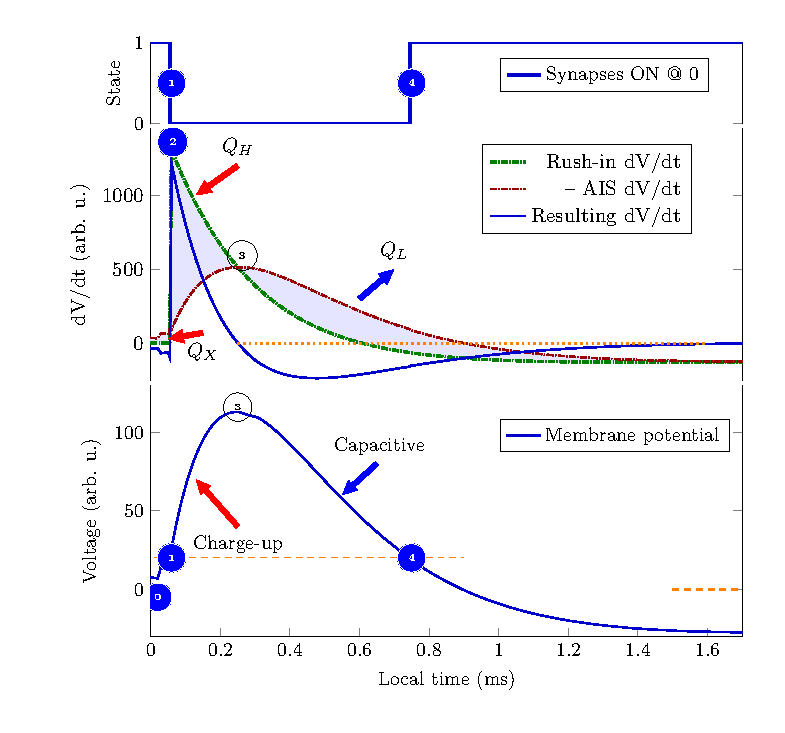
\includegraphics[scale=1]{fig/AP_Artificial_test}
	
	\caption{The physical processes describing the membrane's operation\label{fig:PhysicalProcessesMembrane}. The rush-in $Na^+$ ions instantly increase the membrane's charge, and the membrane's capacity discharges (producing an exponentially decaying voltage derivative). The ions are created at different positions on the membrane, so they take different times to reach the \gls{AIS}, where the current produces a peak in the voltage derivative. The resulting voltage derivative, the sum of the two derivatives (the \gls{AIS} current is outward), drives the oscillator. Its integration produces the membrane potential. When the membrane potential crosses the threshold, it switches the synaptic currents on or off.}
	
\end{figure}

The fundamental difference between the parallel and serial $RC$ circuits is that \textit{the parallel circuit cannot produce output voltage with opposite sign, while the serial one changes the sign of its output
for rising and falling edges of the input voltage}. 
As discussed, the capacitive current, which by definition changes its direction and so 
generates an opposite voltage on the resistor represented by the \gls{AIS}, perfectly describes the so-called "hyperpolarization". It is not the effect of a $K^+$ current: the resting ion channels do not have sufficient conductance.  
Not knowing about the \gls{AIS} leads to assuming that the resting ion channels work also as transient channels (in other words, assuming a parallel $RC$ circuit instead of the serial one, furthermore, that
the output current flows through the membrane instead of the axon). Some $K^+$ current certainly exists; for the magnitude of currents during \gls{AP}, see~\cite{NeuralEnergyConsumption:2017}.


The shape of the output waveform depends on the ratio of the pulse width to the $RC$ time constant. When $RC$ is much larger than the pulse width, the output waveform resembles the input signal, even with a square wave input. (In the case of the neuronal oscillator, the shape of the front side of the spike is similar to the one derived for the rush-in current, while the back side is very prolonged.)

The sudden rush-in of
$Na^+$ ions has (at least) a double effect. 
One effect is that they press the surface of the membrane that
elastically increases its diameter~\cite{NeuronalDeformation:2020}.
 Due to their mutual repulsion,
the ions experience a strong electrical force toward the membrane. It represents an impulse $J=F\,\Delta t$ (N\, s), that enables estimating the time and energy of the 
change the rush-in causes and explains that the energy needed to 
generate an \gls{AP} is suddenly produced electrically, 
and stored temporarily as elastic energy (the neuron produces the required energy in the background, when \gls{ATP} produces ions by hydrolysis under the effect of the electrical field near to membrane); see Appendix~\ref{sec:Physics-Speculations}. 
The case is practically identical to
the deformation of an elastic plate induced by the hydrostatic pressure of a water column. At the beginning, the aluminum plate is suddenly subjected to hydrostatic pressure, and it reaches equilibrium after initial oscillations. The diagram line of the process is shown in the figure
\cite{HydrostaticWaterColumn:2021}, and the method of simulation is discussed in \cite{Hydrostatic_SPHinXsys:2021}. Compare the diagram line to the
gradient in Fig.~\ref{fig:PhysicalProcessesMembrane}, middle inset.


\subsection{Thermodynamics of Action Potential\label{sec:Physics-ThermodynamicsAP}}

 In a way 
demonstrating the need for the non-disciplinary discussion,
we derive the thermodynamic Carnot-cycle of AP from
measuring electrical parameters, calculate its energy consumption and efficiency, interpret the neuron's partially reversible operation and
the long-sought solution to the heat emission/absorption issue.
We defy the claim that science cannot describe life: the underlying physics constrains biological phenomena, including cognitive ones.



\subsubsection{Deriving thermodynamic description\label{sec:Physics-DerivingThermodynamics}}
As the middle inset in Fig.~\ref{fig:PhysicalProcessesMembrane} shows, the sum of the rush-in and \gls{AIS} gradients (plus more gradients if any) controls the generation of the \gls{AP}. During excitation, $Q_X$ energy is fed into the neuron. The rush-in of the $Na^+$ ions injects more $Q_R$ energy, which can be used to generate an \gls{AP}.
It is a kind of potential energy, which is converted in the first 
phase of $AP$ (while the voltage gradient is positive) to the kinetic energy $Q_H$ of \gls{AP}.
When the membrane potential reaches its peak, the gradient reverses, decreasing the potential.  
In the second phase of \gls{AP} (while the voltage gradient is negative)
the neuron harvests $Q_L$ energy.
At the beginning of the transient state, the size of the neuron (due to the increased electrostatic repulsion) slightly increases~\cite{NeuronalDeformation:2020} and stores the energy mainly in the form of elastic energy. The resultant of the electrical, elastic, and thermodynamic forces moves the ions toward the \gls{AIS}. 
 Although part of the energy is dissipated while the ions exit through the \gls{AIS} with their Stokes-Einstein speed, the rest of the energy (the elastic part) is recovered.
 The concentration and potential values change as discussed in connection with Fig.~\ref{fig:RestingPotential4}. The membrane voltage controls synapses as shown in the top inset in Fig.~\ref{fig:PhysicalProcessesMembrane}.
 
\begin{figure}
	\begin{tabular}{cc}
		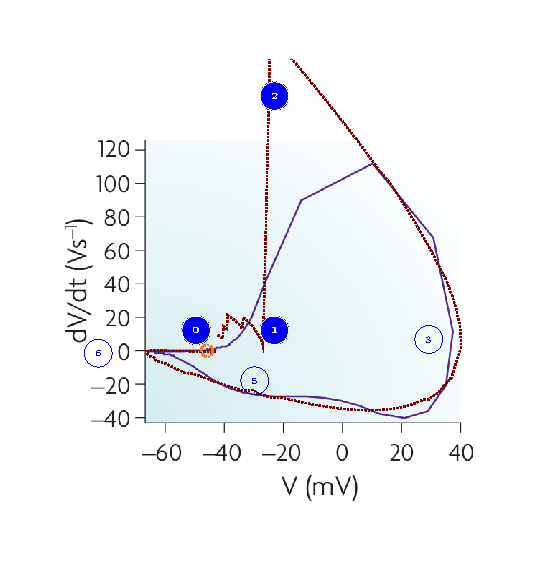
\includegraphics[height=8cm,trim={1.1cm 1.0cm 1cm 0cm },clip]{fig/Bean_V_dV}
		&
		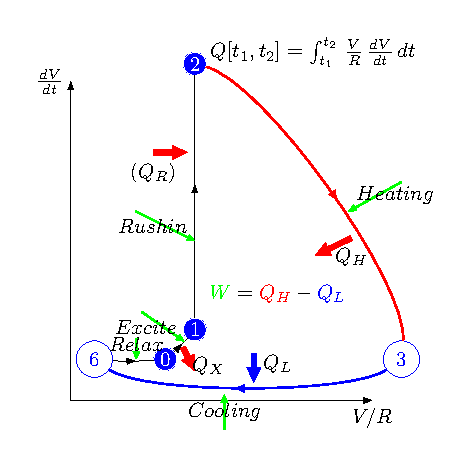
\includegraphics[,trim={1.5cm -0.26cm 0cm 0cm},scale=1]{fig/Carnot}
	\end{tabular}
	\caption{Thermodynamic consequences of the processes shown in Figure~\ref{fig:PhysicalProcessesMembrane} during the generation of an Action Potential. Left: Comparing the measured (broken blue) and theoretical (red dotted) voltage gradient vs voltage phase diagrams~\cite{BeanActionPotential:2007}. 
		Right: Reinterpreting the phase loop in terms of thermodynamics: the “Carnot cycle” (theoretical thermodynamic cycle) of a neuron \label{fig:Carnot} \label{fig:Bean_V_dV}	}
\end{figure}


\begin{figure}
	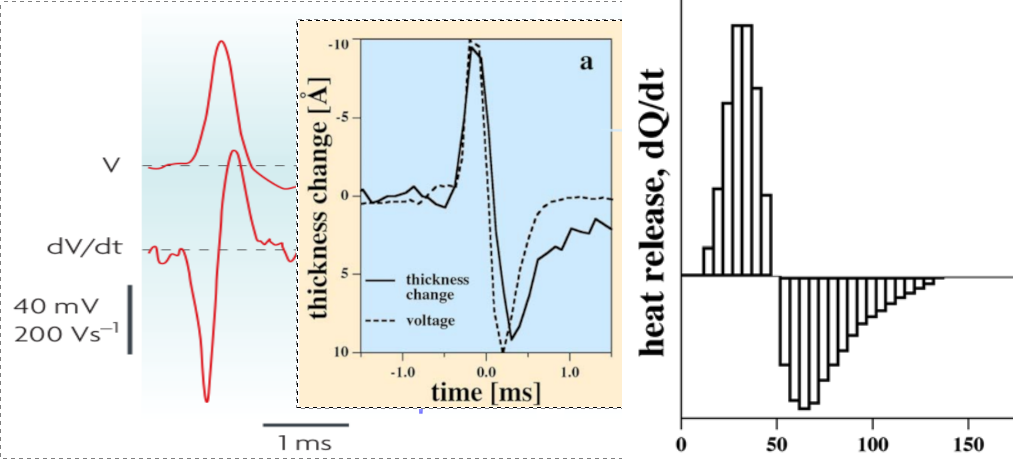
\includegraphics[%,trim={1.5cm 00cm 0cm 0cm},
	scale=1.5]{fig/ElasticityGradientHeimburg.png}
	\caption{The time course of the electrical gradient~\cite{BeanActionPotential:2007} perfectly matches that of the mechanical and thermal changes~\cite{HeimburgPhysikOfNerves:2009}; however, classic theory cannot explain the connection between them~\cite{VeghNonOrdinaryLawsForLife:2025}.
		\label{fig:HeimburgElascticity}
		The experimental $\frac{dV}{dt}$ uses an opposite sign convention.}
\end{figure}

The ‘phase loop’ (how the voltage gradient and membrane voltage correlate; a parametric curve that uses time $t$ as parameter) shown on the left side of Fig.~\ref{fig:Bean_V_dV} represents a strong test of the theoretical line shape: the values of the potential and its gradient are simultaneously compared to the experimentally measured ones. Comparing the experimental and theoretical shapes supports the theory that describes the mutual dependence of voltage and its gradient. Furthermore, it shows that omitting the gradient from the classic theory misled the experiment designers, and the measurement design was wrong: the time interval between recording data points was too long. 
Where the gradient is high and changes quickly (see Fig.~\ref{fig:PhysicalProcessesMembrane}, middle inset), the blue experimental diagram line is roughly broken. The changes in the values are too significant, causing the integration to distort the value and resulting in an inaccurate broken line. In the rush-in region, the theoretical line is even outside the figure's range. Where the gradient change is slow, the measurement points are sufficiently dense, and the theory perfectly describes the experimental data. Neither of the mentioned competing (or other classical) theories can interpret the phenomenon and produce any similar dependence. 

An exciting aspect is that the phase plot in Fig.~\ref{fig:Bean_V_dV}, left side, shows a remarkable resemblance to a specialized thermodynamic Carnot cycle in Fig.~\ref{fig:Bean_V_dV}, right side; and inspires us to interpret the parameters of the "neuronal Carnot machine" (the bent arcs serve only for illustration; they do not follow the path on the left side). 
As discussed in~\cite{HeimburgPhysikOfNerves:2009}, a neuron emits and absorbs heat (energy) in the first and second phases, respectively, of an \gls{AP}; see Fig.~\ref{fig:HeimburgElascticity}.
The experience, alone, defies the classical \gls{HH} mechanism: the leakage current can only emit heat, but not absorb it.
\textit{Laws describing currents of electrons must not be used directly to currents of ions. Neglecting the repelling force between the charge carriers of the ion current, which can be omitted in the case of electron current, leads to entirely wrong conclusions, from the wrong oscillator model to losing the connection between the electrical and mechanical changes, to losing the connection between inanimate and living nature.}
Our theoretical model, unlike the others, can explain that observation quantitatively.

We rescale the horizontal axis by the resistance $R$ of the \gls{AIS} (actually, the horizontal axis is transformed to $I_{AIS}$); thus, the plot becomes a neuronal energy density diagram.
Actually, it corresponds to a usual $P-V$ thermodynamic diagram, 
and we expect that the temperature changes in the same analogy
(we keep the convention of using the letter $V$ to denote both potential and volume).
By integrating the parametric $t$ values of any two points on the diagram ‘circle’ line, we receive the work performed by the neuron.

We consider that the environment in the period ‘Excite’ invests energy $Q_X$ through the neuron’s synapses (increases the membrane’s voltage to the threshold) between [0,1] to open the valves.
 Opening the valves enables the neuron receiving in period ‘Rushin’ energy $Q_R$ by letting in $Na^+$ ions, accelerated by the field across the membrane. Suddenly, the ion concentration and the membrane potential reach their maximum values (given that the current is slow,
 the sudden change generates a smeared and delayed current on the \gls{AIS}, see Fig.~\ref{fig:PhysicalProcessesMembrane}, middle inset). Given that the process is instant, the potential $V$ does not change (no current flows), so the integral [1,2] evaluates to zero (an ‘iso-voltage’ transition). Now the neuron has a high potential to prepare its (already encoded) message (the \gls{AP}).
In terms of electricity, in the first phase (from the threshold potential to the maximum value of the \gls{AP}, where $\frac{dV}{dt}$ is positive), the neuronal power cycle produces a positive heat $Q_H$, given that $\frac{dV}{dt}$ is always positive. 
In the second phase (from the top value of \gls{AP} to where the driving force $\frac{dV}{dt}$ becomes zero again), the neuronal power cycle produces a negative heat $Q_L$, given that $\frac{dV}{dt}$ is always negative; in line with the measurement results shown in Fig.~\ref{fig:HeimburgElascticity}~\cite{HeimburgPhysikOfNerves:2009}. The integral [2,3] provides the “heating” $Q_H$, the energy invested. Similarly, the integral [3,6] provides the “cooling” $Q_L$, representing the energy recovered (assuming no artificial current). 

In terms of thermodynamics, the ions stop in the immediate vicinity of 
the membrane, i.e., initially, the pressure created by their mutual repulsion is present at the inner surface of the sphere (it is a mechanical shock wave). In the positive phase of the damped oscillation, it compresses the fluid in the sphere. In the second phase, in the negative 
phase of oscillation, it decompresses the fluid (sucks back the fluid).
Given that the density of ions in the volume is constant
(the ions' speed is too low to follow those sudden changes),
the electrical and thermodynamic quantities faithfully follow each other.
Measuring electrical potential and mechanical pressure yields disciplinary measurements of the same physical effect.

In the “Relax” phase, $\frac{dV}{dt}$  is (almost) zero, so the corresponding integral evaluates to zero (‘iso-gradient’ transition). In this phase, the neuron must restore its resting state: by using \gls{ATP}, it creates new ions. The difference in the energies of $Q_H$ and $Q_L$ is the net energy used to forward an \gls{AP}; while $Q_X$ is the energy used to perform the computation. The energy $Q_X$ is an approximate value: as shown in Fig.~\ref{fig:PhysicalProcessesMembrane}, at the time of re-opening the synaptic inputs, the membrane can be above or below the resting potential, which actually means a neuron-level memory. In this sense, adjacent neural spikes can borrow energy from each other (which explains why the spikes in a burst behave differently). The energy $Q_R$ is produced by the \gls{ATP} hydrolysis in parallel with the 'primary processes' described above, and the produced ions are acquired on the condenser plates, thus restoring the resting potential and providing potential energy for the forthcoming spikes. 

From Fig.~\ref{fig:Carnot}, after recalibration (with $R_{AIS}=10^7$ Ohm), one %gets an energy diagram, and 
can estimate (by approximating roughly the area under the arcs by triangles, in units of $10^{-7} [J]$), $Q_H =5.2, Q_L=1.8, W=3.4, Q_X=0.2$. That is, according to the "phase plot"~\cite{BeanActionPotential:2007}, the neuron operates with an efficiency around 65\%, and approximately 3\% of the energy is derived from the upstream neurons. The values (without using data from dedicated measurements) agree excellently with the measured~\cite{NeuralEnergyConsumption:2017} values $W=2.5$ and 74\%; furthermore, the $Q_X$:total ratio $1:35$, derived by measuring the direct energy consumption~\cite{EnergyNeuralCommunication:2021}.
\textit{An interesting proof that the two disciplines see the same physical effect, that electrical parameters can measure the thermodynamic efficiency.} The invested energy can be safely estimated from the work the rush-in charge performs given that the energy is almost entirely stored as elastic potential energy due to the enormous elasticity modulus

%In our model, the $Na^+$ rush-in increases the potential, the concentration, the pressure (due to electrical repulsion; so it changes the membrane's capacity), and the volume (since the membrane is elastic), so a multi-dimensional Carnot diagram could describe the state accurately (although the invested energy can be safely estimated from the work the charge performs given that the energy is almost entirely stored as elastic potential energy due to the enormous elasticity modulus). Furthermore, all parameters have a time course. It is not possible to provide a more accurate estimation without a true multi-physics simulation. However, the approach is promising. 



\subsubsection{Neural entropy\label{sec:HeatEntropy}}
The theoretical diagram line in Fig.~\ref{fig:Carnot}, based on the presented correct physical model, might serve as a good starting point for interpreting \textit{entropy} for neuronal operation, again in analogy with the Carnot cycle; although the charge of the ions (the macroscopic current) complicates the process. Furthermore, material convection happens in
different ill-defined volume parts of the membrane in different directions. Initially, in the resting state, the ions are in a (relatively) disordered state. After the rush-in, in the dynamic layer, the ions have a highly ordered macroscopic speed (see Stokes-Einstein speed, the gradually changing gradients, and the finite speed) component toward the \gls{AIS}. In the layer, the maximum ordered state is reached when the voltage drop on the \gls{AIS} reaches its peak value (the current is slow). Then, the ions slow down, and at zero voltage gradient, they reach again a minimally ordered state. After that, due to the 'capacitive current', the current reverses its direction, and the backward current again represents an ordered state.  
Perhaps the latter-mentioned negative contribution is the one referred to as ‘negative entropy’ when describing life in terms of thermodynamic processes? We must be aware that, in the background, energy-producing processes are at work, involving the ordered transport of material. Considering the neuron, based only on the described primary processes, would be a mistake.

The above discussion might help in understanding the \textit{physical entropy}
in the neuron; although, as discussed above, there are issues with calculating partial derivatives (and so: deriving entropy from the Gibbs energy of the system) and with the applicability of Boltzmann assumptions to ensembles of ions. However, the \textit{information entropy} is different. 
As our discussion underpins, the "information" arrives at the neuronal inputs as charge carriers, and the time course of the input currents, in cooperation with the neural environment and the neuron itself, carries the information in some form. 
The information is distributed in space and time~\cite{VeghNeuralShannon:2022, VeghChannelCapacity:2023}, so we can be sure that using the pulse count as a measure of neural information is wrong. We must distinguish the \textit{carrier of the information}, the ion, and the \textit{information content} that its temporal appearance carries. After having the correct physical model of operation, we have a chance to gain more knowledge about how the
information is encoded in the spatially and temporally distributed
observable signals; furthermore, we have greater hope of understanding neural information processing, including the brain's entropy handling.

